\documentclass[11pt,a4paper]{report}

% --- Pacotes ---
\usepackage[utf8]{inputenc}
\usepackage[T1]{fontenc}
\usepackage{lmodern}
\usepackage[portuguese]{babel}
\usepackage{graphicx}
\usepackage[margin=2.5cm]{geometry}
\usepackage{hyperref}
\usepackage{setspace}
\usepackage{float}
\usepackage{titlesec}
\usepackage{array}
\usepackage{tikz}
\usetikzlibrary{arrows.meta,positioning,shapes.geometric,fit}

\onehalfspacing

\begin{document}

% ================= CAPA =================
    \begin{titlepage}
        \centering
        
\includegraphics[width=0.80\textwidth]{images.png}\par
        \vspace{1.2cm}

        {\scshape\Large Instituto Superior de Engenharia de Lisboa \par}
        \vspace{2cm}

        {\Huge\bfseries OmniAI Gateway\par}
        \vspace{0.4cm}
        {\LARGE Relatório Final de Projeto\par}

        \vspace{2.5cm}

        \rule{0.8\textwidth}{0.4pt}
        \vspace{1cm}

        {\large
            \begin{tabular}{c}
                \textbf{Guilherme Coutinho} \\
                Nº 50467 \\
                A50467@alunos.isel.pt \\
                \\
                \textbf{André Nunes} \\
                Nº 51766 \\
                A51766@alunos.isel.pt \\
            \end{tabular}
        }

        \vspace{1.5cm}

        {\large
        \textbf{Orientador:} Pedro Félix \\
        pedro.felix@isel.pt
        }

        \vfill

        {\large
        Engenharia Informática e de Computadores \\
        \vspace{0.3cm}
        \today
        }

    \end{titlepage}

% ================= ELEMENTOS PRÉ-TEXTUAIS =================
    \begin{abstract}
        A ausência de um protocolo comum na comunicação com Modelos de Linguagem de Grande Escala (LLMs) obriga as aplicações a integrarem diferentes interfaces de acesso e implementações particulares para a invocação de ferramentas externas. Para resolver esta fragmentação tecnológica, este projeto propõe o desenvolvimento do \textbf{OmniAI SDK}, um \textit{Software Development Kit} construído em Kotlin Multiplatform (KMP). Baseado nos princípios da Arquitetura Hexagonal (\textit{Ports and Adapters}), o SDK isola a lógica de domínio e suporta a comunicação bidirecional compatível com os padrões das APIs de referência, nomeadamente OpenAI, Anthropic e Gemini. O núcleo do sistema implementa uma \textit{pipeline} extensível e configurável, inspirada no modelo de filtros de Servlets, que executa \textit{interceptors} pré-construídos para autorização, autenticação, métricas, \textit{rate limiting}, \textit{circuit breaker} e \textit{fallback}. Adicionalmente, o SDK integra um MCP Broker, permitindo o registo dinâmico de ferramentas externas através de configuração. Distribuído de forma multiplataforma para ambientes JVM, via Maven, e Node.js/TypeScript, via NPM, o SDK foi validado através da construção da \textbf{OmniAI Gateway}, uma aplicação final que consome a biblioteca para instanciar rapidamente uma Gateway. A avaliação demonstra que a solução minimiza o acoplamento tecnológico e o esforço de integração, garantindo resiliência, escalabilidade e centralização na gestão de modelos de IA.
    \end{abstract}

    \renewcommand{\abstractname}{Abstract}
    \begin{abstract}
        The lack of a common protocol for communicating with Large Language Models
        (LLMs) forces applications to integrate different access interfaces and
        specific implementations for invoking external tools. To address this
        technological fragmentation, this project proposes the development of the OmniAI SDK, a
        Development Kit built on Kotlin Multiplatform (KMP). Based on the principles of the
        Hexagonal Architecture (Ports and Adapters), the SDK isolates the domain logic and supports
        bidirectional communication compatible with the standards of reference APIs, namely OpenAI,
        Anthropic, and Gemini. The system’s core implements an extensible and configurable pipeline, inspired
        by the Servlet filter model, which executes pre-built interceptors for authorization, au-
        thentication, metrics, rate limiting, circuit breaker, and fallback. Additionally, the SDK integrates an
        MCP Broker, enabling the dynamic registration of external tools through configuration.
        Distributed across multiple platforms for JVM environments via Maven and Node.js/TypeScript
        via NPM, the SDK was validated through the development of the OmniAI Gateway, an end-user
        application that leverages the library to rapidly instantiate a Gateway. The evaluation demonstrates that
        the solution minimizes technological coupling and integration effort, ensuring resilience,
        scalability, and centralization in AI model management.
    \end{abstract}

    \tableofcontents
    \listoffigures
    \newpage

% ================= CAPÍTULOS DO RELATÓRIO =================

    \chapter{Introdução}

    \section{Contexto}
    Os Modelos de Linguagem de Grande Escala (\textit{Large Language Models -- LLMs}) \cite{ibm_llm_topics} tornaram-se componentes relevantes no desenvolvimento de aplicações baseadas em inteligência artificial. Um LLM é um modelo treinado com grandes volumes de texto, capaz de interpretar linguagem natural, gerar respostas e apoiar tarefas como sumarização, classificação, programação assistida, pesquisa semântica e interação com sistemas externos.

    É possível distinguir duas fases principais no ciclo de vida de um modelo: treino e inferência. O treino corresponde ao processo de aprendizagem a partir de grandes conjuntos de dados, exigindo elevados recursos computacionais. A inferência corresponde à utilização do modelo já treinado para gerar respostas a novos pedidos. Atualmente, a maioria das aplicações integra LLMs através de APIs de inferência disponibilizadas por fornecedores externos.

    A comunicação com estas APIs é normalmente realizada em JSON, tanto nos pedidos como nas respostas. Antes de serem processados pelos modelos, os textos são convertidos em \textit{tokens}, pequenas unidades de informação que permitem ao modelo representar e manipular sequências de entrada e saída \cite{nvidia_tokens}. Como a resposta é gerada de forma incremental, muitas APIs suportam \textit{streaming}, permitindo enviar fragmentos da resposta ao cliente à medida que são produzidos.

    Existem vários fornecedores relevantes, incluindo OpenAI \cite{openai_api}, Anthropic \cite{anthropic_api}, Google Gemini \cite{google_gemini_api} e Groq \cite{groq_api}. Embora todos disponibilizem APIs HTTP e estruturas JSON, cada fornecedor define contratos próprios, campos específicos, regras de autenticação e modelos distintos para \textit{tool calling}. A integração direta com vários fornecedores obriga, por isso, as aplicações a conhecerem detalhes internos de cada API.

    Ao mesmo tempo, o uso de LLMs evoluiu de interações simples para sistemas baseados em agentes (\textit{agentic workflows}) \cite{ibm_agentic_workflows}. Nestes cenários, o modelo não se limita a devolver texto; pode decidir invocar ferramentas externas, interpretar resultados intermédios e produzir uma resposta final com base nesses dados. O \textit{Model Context Protocol} (MCP) surgiu como proposta de normalização para a comunicação entre modelos, aplicações e ferramentas externas \cite{mcp_protocol}.

    \section{Motivação e Definição do Problema}

    \begin{figure}[H]
        \centering
        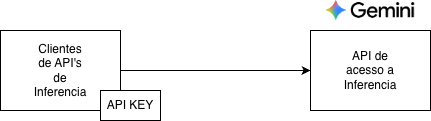
\includegraphics[width=0.9\textwidth]{P1.png}
        \caption{Acoplamento direto entre clientes e um fornecedor de inferência}
        \label{fig:p1}
    \end{figure}
    \begin{figure}[H]
        \centering
        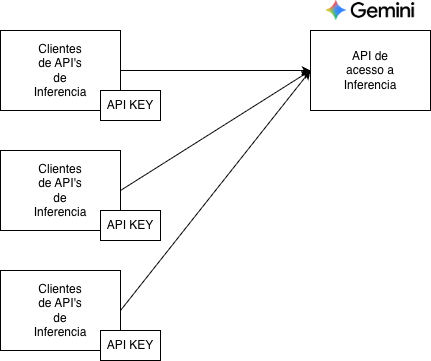
\includegraphics[width=0.9\textwidth]{P2.png}
        \caption{Multiplicação de integrações diretas com vários fornecedores}
        \label{fig:p2}
    \end{figure}
    \begin{figure}[H]
        \centering
        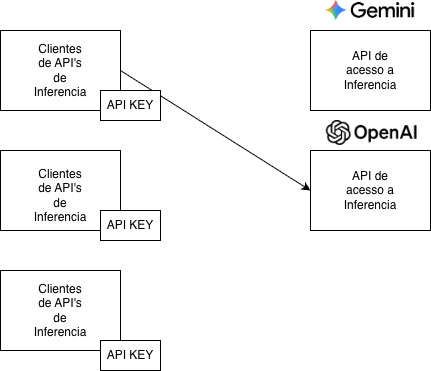
\includegraphics[width=0.9\textwidth]{P3.png}
        \caption{Cliente trocar de fornecedor}
        \label{fig:p3}
    \end{figure}

    As Figuras \ref{fig:p1}, \ref{fig:p2} e \ref{fig:p3} ilustram o acoplamento direto entre clientes e fornecedores de inferência, bem como a dificuldade que os clientes tem em trocar de fornecedor devido a todo acoplamento que existe

    A existência de múltiplos fornecedores de LLMs e a ausência de um protocolo comum implicam
    diferentes interfaces de acesso aos modelos, estruturas específicas de pedidos e respostas, modelos distintos de contabilização de tokens, custos variáveis e implementações particulares para invocação de funções externas (ver Figuras \ref{fig:p1}--\ref{fig:p3}). Por exemplo, a API OpenAI organiza a interação em torno de chat completions e tool calls; a Anthropic utiliza uma arquitetura baseada em messages e blocos de conteúdo; e a Gemini estrutura a geração através de contents, parts, function declarations e configurações de geração próprias.

    Estas diferenças criam acoplamento entre as aplicações cliente e os fornecedores. Sempre que uma aplicação pretende trocar de modelo, suportar mais do que um fornecedor, adicionar um mecanismo de \textit{fallback} ou integrar ferramentas externas, torna-se necessário duplicar lógica de tradução, autenticação, tratamento de erros e interpretação de respostas. Esta duplicação aumenta a complexidade e dificulta a evolução do sistema, um problema recorrente em sistemas que combinam lógica de aplicação com integrações externas especializadas \cite{ml_code_smells,ml_code_smells1}.

    Para além da fragmentação dos contratos, existem preocupações operacionais e de segurança. Uma aplicação que comunica diretamente com vários fornecedores precisa de gerir chaves de API, quotas, limites de utilização, métricas, auditoria, políticas de acesso e proteção contra falhas de terceiros. Sem uma camada intermédia, estas preocupações ficam espalhadas por vários pontos do sistema, tornando mais difícil aplicar regras consistentes de autenticação, autorização, observabilidade e resiliência.

    O problema central deste projeto é, assim, a ausência de uma camada de abstração capaz de separar as aplicações cliente das particularidades de cada fornecedor de LLMs, mantendo simultaneamente suporte para segurança, monitorização, \textit{tool calling} e integração dinâmica com ferramentas externas.

    \section{Objetivos e Proposta de Solução}
    \begin{figure}[H]
        \centering
        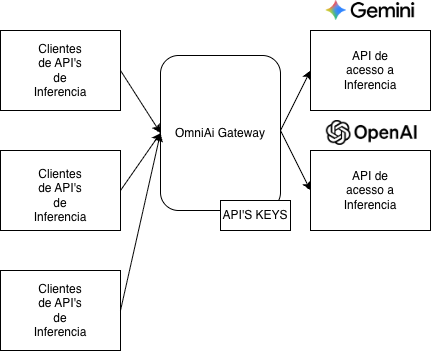
\includegraphics[width=0.9\textwidth]{P4.png}
        \caption{Centralização com OmniAI Gateway}
        \label{fig:p4}
    \end{figure}

    A solução proposta evoluiu para a construção de um \textbf{OmniAI SDK}, isto é, uma biblioteca reutilizável que permite instanciar uma \textbf{OmniAI Gateway}. A Gateway funciona como ponto de entrada único para aplicações cliente, centralizando o acesso a APIs de inferência, ferramentas externas e mecanismos transversais de segurança e operação. Esta abordagem aproxima-se do padrão de API Gateway \cite{api_gateway_design} e, no contexto específico de modelos de IA, do padrão de AI Gateway enquanto camada centralizada de acesso a modelos \cite{ai_gateway_pattern,karl_ai_gateway}. Embora existam soluções relacionadas, como LiteLLM e OpenRouter \cite{litellm,openrouter}, o foco deste projeto está na construção de um SDK extensível, configurável e integrado com uma Gateway final própria.

    O SDK foi desenvolvido em Kotlin Multiplatform, permitindo partilhar o núcleo de domínio entre targets diferentes e preparar a distribuição para JVM e JavaScript/Node.js \cite{kotlin_multiplatform}. Esta decisão torna possível disponibilizar a biblioteca em ecossistemas distintos: via Maven para aplicações JVM/Kotlin e via NPM para ambientes Node.js/TypeScript.

    A arquitetura do SDK foi organizada segundo os princípios da Arquitetura Hexagonal, também conhecida como \textit{Ports and Adapters} \cite{hexagonal_ports}. O domínio comum fica isolado de contratos externos, enquanto os \textit{inbound adapters} traduzem pedidos de clientes compatíveis com OpenAI, Anthropic ou Gemini para o modelo comum, e os \textit{outbound adapters} traduzem o modelo comum para chamadas reais aos fornecedores.

    Para tornar a solução configurável e escalável, foi criada uma \textit{pipeline} interna de \textit{interceptors}, inspirada no modelo de filtros de Servlets \cite{servlet_filterchain}. Esta \textit{pipeline} permite executar comportamentos transversais antes e depois da chamada ao fornecedor, incluindo autenticação, autorização, métricas, \textit{rate limiting}, \textit{circuit breaker}, \textit{fallback} e \textit{logging}. Por fim, a integração com MCP permite gerir ferramentas externas de forma separada da lógica de inferência.

    \section{Estrutura do Documento}
    Este documento encontra-se estruturado da seguinte forma. O Capítulo 2 apresenta o estudo prévio das APIs de inferência e do MCP, bem como a modelação do domínio comum. O Capítulo 3 descreve a arquitetura do sistema, incluindo a separação em módulos e a aplicação da Arquitetura Hexagonal. O Capítulo 4 detalha a implementação técnica do SDK, da \textit{pipeline}, dos \textit{interceptors}, do MCP Broker e da Gateway final. O Capítulo 5 apresenta provas de conceito e validações realizadas. Por fim, o Capítulo 6 sintetiza as conclusões e identifica trabalho futuro.

    \chapter{Estudo Prévio e Modelação de Domínio}

    \section{Análise das APIs de Inferência}
    O estudo inicial comparou APIs de inferência compatíveis com os fornecedores OpenAI, Anthropic e Gemini, bem como execuções locais através de ambientes compatíveis, como Ollama. Esta análise teve como objetivo identificar conceitos comuns e divergências estruturais relevantes para a criação de um domínio unificado.

    A API OpenAI organiza o pedido em torno de um campo \texttt{model}, uma lista \texttt{messages}, parâmetros de geração e, opcionalmente, uma lista de \texttt{tools}. A autenticação é feita por \texttt{Authorization: Bearer <token>}. O \textit{tool calling} devolve chamadas em \texttt{tool\_calls}, contendo identificador, nome da função e argumentos serializados em JSON. O \textit{streaming} é baseado em eventos incrementais, onde cada fragmento contém \texttt{delta} com conteúdo textual ou partes da chamada de ferramenta.

    A API Anthropic utiliza a arquitetura de \textit{messages}. O campo \texttt{max\_tokens} é obrigatório, as instruções de sistema são fornecidas num campo próprio e o conteúdo pode ser uma string simples ou uma lista de blocos estruturados. As ferramentas são descritas através de \texttt{name}, \texttt{description} e \texttt{input\_schema}. Quando o modelo decide usar uma ferramenta, a resposta inclui blocos \texttt{tool\_use} e o ciclo continua com a devolução de blocos \texttt{tool\_result}.

    A API Gemini utiliza \texttt{contents} compostos por \texttt{parts}. O mesmo modelo de conteúdo suporta texto, multimodalidade, chamadas de função e respostas de função. As ferramentas são disponibilizadas através de \texttt{functionDeclarations}; as configurações de geração são agrupadas em \texttt{generationConfig}; e existem particularidades como \textit{thought signatures}, \texttt{thinkingConfig} e parâmetros de segurança. Esta API evidencia a dificuldade de criar uma normalização completa, porque alguns conceitos não têm correspondência direta nos outros fornecedores.

    Desta análise resultaram três conclusões principais. Primeiro, existe um conjunto mínimo comum que pode ser representado por mensagens, papéis, conteúdo, configuração de geração, ferramentas e respostas. Segundo, cada fornecedor contém extensões que não devem ser descartadas, pelo que o domínio precisa de um mecanismo de opções específicas. Terceiro, o suporte a \textit{streaming} exige eventos comuns que preservem a ordem e o significado dos fragmentos recebidos.

    \section{Model Context Protocol (MCP)}
    O \textit{Model Context Protocol} define uma arquitetura cliente-servidor para expor ferramentas, recursos e \textit{prompts} a aplicações baseadas em modelos \cite{mcp_protocol}. No contexto deste projeto, o MCP é relevante porque separa a definição e execução de ferramentas da API de inferência usada em cada pedido.

    A solução proposta integra um \textbf{MCP Broker}, responsável por registar ferramentas externas e disponibilizá-las ao sistema de forma uniforme. A intenção de desenho é permitir que ferramentas sejam adicionadas dinamicamente através de ficheiros de configuração, nomeadamente YAML, evitando a necessidade de recompilar a Gateway sempre que uma nova ferramenta é disponibilizada. A implementação atual do módulo \texttt{mcp-broker} inclui modelos de domínio para ferramentas, recursos e \textit{prompts}, geração de esquemas JSON e um \textit{builder} para configuração de servidores MCP com transporte \texttt{stdio}, SSE ou WebSocket.

    \section{Definição do Domínio}
    A modelação de domínio do OmniAI SDK foi definida a partir dos conceitos comuns identificados no estudo das APIs. O pedido comum é representado por \texttt{CommonRequest}, contendo fornecedor, modelo, mensagens, \textit{system prompt}, configuração de geração, ferramentas, escolha de ferramenta, indicação de resposta JSON e opções específicas do fornecedor.

    As mensagens são representadas por \texttt{CommonRequestMessage}, com um papel comum e uma lista de partes de conteúdo. Esta abordagem permite representar mensagens simples, conteúdos multimodais, resultados de ferramentas e argumentos estruturados sem prender o domínio a um formato de API específico.

    A resposta comum é representada por \texttt{CommonResponse} no caso síncrono e por \texttt{CommonResponseEvent} no caso de \textit{streaming}. A separação entre resposta final e eventos incrementais permite suportar APIs que devolvem um objeto completo e APIs que produzem uma sequência de eventos. Os eventos comuns incluem início de resposta, início de escolha, fragmentos de texto, início de chamada de ferramenta, fragmentos de argumentos, utilização de tokens, conclusão e erro.

    Para preservar extensibilidade, o domínio utiliza estruturas como \texttt{TypedMap} e campos de opções específicas. Assim, dados que não fazem parte do mínimo comum, como parâmetros avançados de Gemini ou Anthropic, podem atravessar a \textit{pipeline} sem contaminar o núcleo do modelo.

    \chapter{Arquitetura e Desenho do Sistema}

    \section{Arquitetura Top-Level}
    A arquitetura top-level organiza o sistema em três zonas principais: clientes externos, OmniAI Gateway/SDK e fornecedores de inferência ou ferramentas. A Gateway expõe endpoints compatíveis com contratos conhecidos, recebe pedidos de aplicações cliente, aplica a \textit{pipeline} de \textit{interceptors} e encaminha a chamada para o fornecedor adequado.

    \begin{figure}[H]
        \centering
        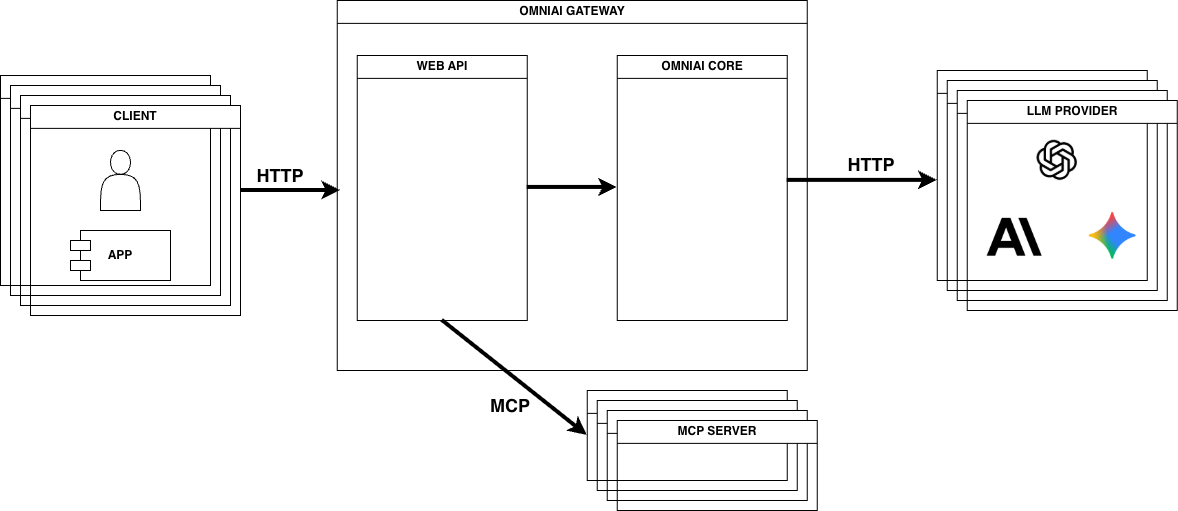
\includegraphics[width=0.9\textwidth]{arquiteturaF.png}
        \caption{Diagrama da Arquitetura Top-Level do Sistema}
        \label{fig:top-level}
    \end{figure}

    \begin{figure}[H]
        \centering
        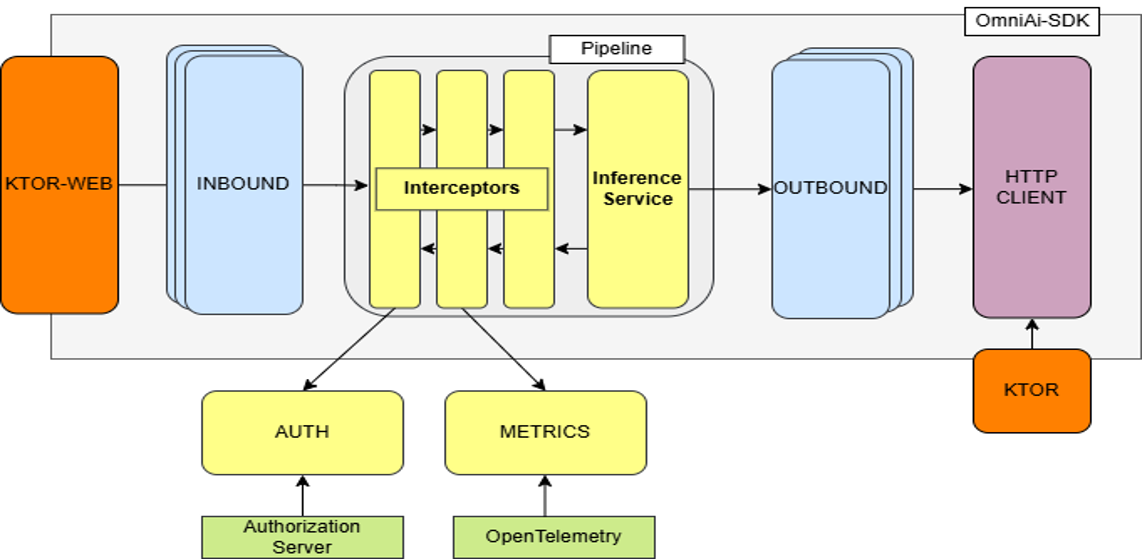
\includegraphics[width=0.95\textwidth]{arquitet}
        \caption{Visão da integração entre Ktor, inbounds, pipeline, interceptors, outbounds e HTTP client no OmniAI SDK}
        \label{fig:arquitet-sdk}
    \end{figure}

    Esta organização permite que aplicações já compatíveis com APIs existentes possam ser integradas com esforço reduzido. Por exemplo, uma aplicação preparada para a API Anthropic pode alterar o seu \texttt{baseURL} para apontar para a OmniAI Gateway, mantendo o contrato esperado pelo cliente. O mesmo princípio aplica-se a clientes compatíveis com OpenAI e, parcialmente, a clientes que usam endpoints Gemini.

    \section{Arquitetura Hexagonal (Ports \& Adapters)}
    A Arquitetura Hexagonal foi usada para separar a lógica de domínio dos detalhes de transporte e dos contratos externos. No OmniAI SDK, esta separação aparece através de \textit{ports} internos e \textit{adapters} específicos.

    \subsection{Contracts}
    Os módulos \texttt{contracts:openai}, \texttt{contracts:anthropic} e \texttt{contracts:gemini} modelam os formatos de pedido, resposta e eventos de cada fornecedor. Estes contratos representam a fronteira entre o mundo externo e o domínio comum. Esta camada evita que os detalhes de JSON de cada API se espalhem pelo núcleo do sistema.

    \subsection{Inbounds}
    Os \textit{inbound adapters} recebem pedidos no formato do cliente e traduzem-nos para \texttt{CommonRequest}. Existem adapters para OpenAI, Anthropic e Gemini. Estes adapters permitem que a Gateway exponha APIs compatíveis com diferentes padrões de mercado, mesmo que internamente o processamento seja feito por uma única representação.

    \subsection{Outbounds}
    Os \textit{outbound adapters} fazem o caminho inverso: recebem um \texttt{CommonRequest} e transformam-no no contrato do fornecedor real. A implementação atual inclui adapters outbound para OpenAI, Anthropic e Gemini. Estes adapters também traduzem as respostas e eventos de \textit{streaming} de volta para o domínio comum.

    \subsection{Dispatcher}
    O \texttt{DispatcherPort} representa o ponto terminal da \textit{pipeline}. A implementação de despacho pode ser simples, escolhendo um fornecedor configurado, ou evoluir para estratégias mais avançadas, como seleção por custo, latência, disponibilidade, plano do cliente ou política de \textit{fallback}. No projeto, o módulo \texttt{dispatcher} inclui um \textit{router} simples e um \texttt{PipelineBackedDispatcher}.

    \section{Ecossistema do SDK}
    O SDK está organizado como um projeto Gradle multi-módulo. Os módulos principais incluem \texttt{core}, \texttt{contracts}, \texttt{inbound}, \texttt{outbound}, \texttt{interceptors}, \texttt{mcp-broker}, \texttt{dispatcher}, \texttt{gateway-client} e \texttt{gateway-ktor-server}. Esta divisão permite evoluir cada área com responsabilidades claras.

    O módulo \texttt{gateway-client} disponibiliza uma DSL para montar uma Gateway. A aplicação final pode declarar os \textit{inbounds}, os \textit{outbounds}, os \textit{interceptors} e a configuração de segurança. O módulo \texttt{gateway-ktor-server} fornece o adapter HTTP/Ktor que expõe as rotas compatíveis com os contratos externos.

    A aplicação \texttt{OmniAiGateway} foi desenvolvida como validação do SDK. Em vez de reimplementar a lógica de roteamento e tradução, consome o SDK através de um \textit{composite build} do Gradle, usando \texttt{includeBuild("../OmniAi-SDK")}. Esta opção facilita o desenvolvimento local, porque alterações ao SDK podem ser testadas pela Gateway sem publicação intermédia em Maven.

    \chapter{Implementação e Evolução Técnica}

    \section{Stack Tecnológica e Metodologias}
    O SDK foi desenvolvido em Kotlin Multiplatform com targets JVM e JavaScript/Node.js. A escolha de KMP permite partilhar o domínio, contratos e parte da lógica de \textit{pipeline} entre ambientes diferentes, mantendo implementações específicas quando necessário. A camada HTTP utiliza Ktor, e a serialização dos contratos é baseada em Kotlinx Serialization.

    O projeto usa Gradle com estrutura multi-módulo e \textit{composite builds} \cite{gradle_composite_builds}. A Gateway final é um projeto Ktor separado que inclui o SDK localmente durante o desenvolvimento. Esta organização reduz o ciclo de feedback entre alterações à biblioteca e validação numa aplicação real.

    As ferramentas de desenvolvimento incluíram Git para controlo de versões, IntelliJ IDEA como ambiente principal de desenvolvimento e agentes de apoio à programação, como Antigravity, para acelerar exploração e geração de código. Estes agentes foram usados como apoio ao desenvolvimento, mantendo a validação no código, nos testes e nos cenários executados.

    \section{A Primeira Iteração da Gateway}

    A primeira iteração do projeto consistiu na construção direta de uma Gateway HTTP responsável por receber pedidos de clientes e encaminhá-los para fornecedores de inferência. Nesta fase inicial, o objetivo principal era validar rapidamente a viabilidade da solução, testar a comunicação com diferentes APIs e compreender as diferenças práticas entre os contratos da OpenAI, Anthropic e Gemini.

    Esta abordagem permitiu obter resultados rápidos, mas revelou limitações importantes à medida que o sistema cresceu. A lógica de tradução entre formatos, a configuração dos fornecedores, a autenticação, o tratamento de erros e o encaminhamento dos pedidos começaram a ficar concentrados na própria aplicação Gateway. Como consequência, cada novo fornecedor ou funcionalidade transversal exigia alterações diretas no mesmo conjunto de componentes, aumentando o acoplamento e dificultando a evolução do projeto.

    Além disso, tornou-se claro que a Gateway não deveria ser apenas uma aplicação final, mas sim uma consequência de uma biblioteca reutilizável. O problema identificado no projeto não era apenas criar uma Gateway específica, mas fornecer uma base extensível para construir gateways de IA com diferentes configurações, fornecedores e políticas operacionais.

    A partir desta constatação, a arquitetura foi reorganizada. O \textbf{OmniAI SDK} passou a concentrar os elementos reutilizáveis do sistema, incluindo o domínio comum, os contratos, os adapters de entrada e saída, a pipeline de interceptors e os mecanismos de configuração. Por outro lado, a \textbf{OmniAI Gateway} passou a ser uma aplicação concreta construída sobre o SDK, responsável por carregar configuração, instanciar os componentes necessários e expor os endpoints HTTP.

    Esta separação trouxe maior modularidade e reutilização. A Gateway final deixou de conter a lógica principal de integração com fornecedores e passou a consumir o SDK como uma camada de infraestrutura. Desta forma, outras aplicações podem usar o mesmo SDK para criar gateways próprias, com diferentes fornecedores, políticas de autenticação, mecanismos de observabilidade ou estratégias de roteamento.

    A evolução natural foi separar a Gateway final da biblioteca base. O OmniAI SDK passou a concentrar o domínio, os contratos, os adapters e a \textit{pipeline}; a OmniAI Gateway passou a ser uma aplicação que consome essa biblioteca. Esta separação tornou a solução mais reutilizável: outras aplicações podem usar o SDK para criar gateways próprias, com configurações e políticas diferentes.

    \section{Decisões de Desenho e Alternativas Descartadas}
    Em engenharia de software, a análise de \textit{trade-offs} e a delimitação do âmbito são fundamentais. Durante a fase de desenho arquitetural, foram avaliadas abordagens técnicas que acabaram por ser descartadas de forma consciente, priorizando a estabilidade e o foco no domínio principal da Gateway:

    \begin{itemize}
        \item \textbf{Geração de Bridges com KSP (Kotlin Symbol Processing):} Inicialmente, ponderou-se a utilização de KSP para gerar automaticamente as \textit{bridges} de comunicação multiplataforma entre o código Kotlin e o ecossistema TypeScript/Node.js. Contudo, após análise, concluiu-se que a complexidade de configuração do KSP e o tempo de desenvolvimento necessário para mapear todos os \textit{edge cases} de tipagem teriam um impacto severo no planeamento. Optou-se por uma exportação manual controlada (usando \texttt{@JsExport}), garantindo a entrega da biblioteca dentro do prazo estipulado.
        \item \textbf{Injeção Automática de Ferramentas via SSE:} Foi também avaliada a possibilidade de a Gateway intercetar automaticamente os pedidos de \textit{tool calling} durante fluxos de \textit{streaming} (\textit{Server-Sent Events} - SSE) e injetar as respostas das ferramentas sem que o cliente tivesse de gerir esse ciclo. No entanto, a gestão de estado complexa necessária para suspender, intercetar e retomar um \textit{stream} de \textit{tokens} de forma concorrente e segura introduziria uma enorme complexidade na primeira versão do SDK. Esta capacidade foi documentada como trabalho futuro, mantendo o roteamento base resiliente e previsível.
    \end{itemize}

    \section{Evolução Arquitetural: De \textit{Inference Service} a \textit{Dispatcher}}
    A primeira iteração do sistema consistiu numa Gateway monolítica. A lógica de comunicação, a tradução de contratos e o roteamento estavam fortemente acoplados num único componente designado por \texttt{InferenceService}.

    Embora esta estratégia tenha permitido validar rapidamente a comunicação com os fornecedores (OpenAI, Anthropic e Gemini), rapidamente se identificou um problema de escalabilidade de código: o serviço estava a tornar-se num \textit{God Object}, violando o Princípio de Responsabilidade Única (SRP). Cada nova API ou funcionalidade transversal (como métricas ou \textit{rate limiting}) exigia alterações diretas neste serviço central.

    Para resolver este acoplamento, a arquitetura sofreu uma refatorização profunda. O serviço monolítico foi decomposto e substituído por um \textit{Dispatcher} central (\texttt{DispatcherPort}). A responsabilidade deste \textit{Dispatcher} passou a ser única e exclusiva: coordenar o envio do pedido para o \textit{Outbound Adapter} correto. Simultaneamente, toda a lógica transversal que congestionava o sistema foi extraída para uma \textit{pipeline} configurável de \textit{interceptors}.

    \section{Evolução para a Pipeline de Interceptors}
    Para evitar que autenticação, autorização, métricas, limites e \textit{fallback} ficassem embutidos nos adapters ou no dispatcher, foi criada uma \textit{pipeline} de \textit{interceptors}. A ideia é semelhante ao modelo de filtros de Servlets: cada interceptor recebe um contexto, decide se continua a cadeia e pode observar ou alterar o resultado.

    \begin{figure}[H]
        \centering
        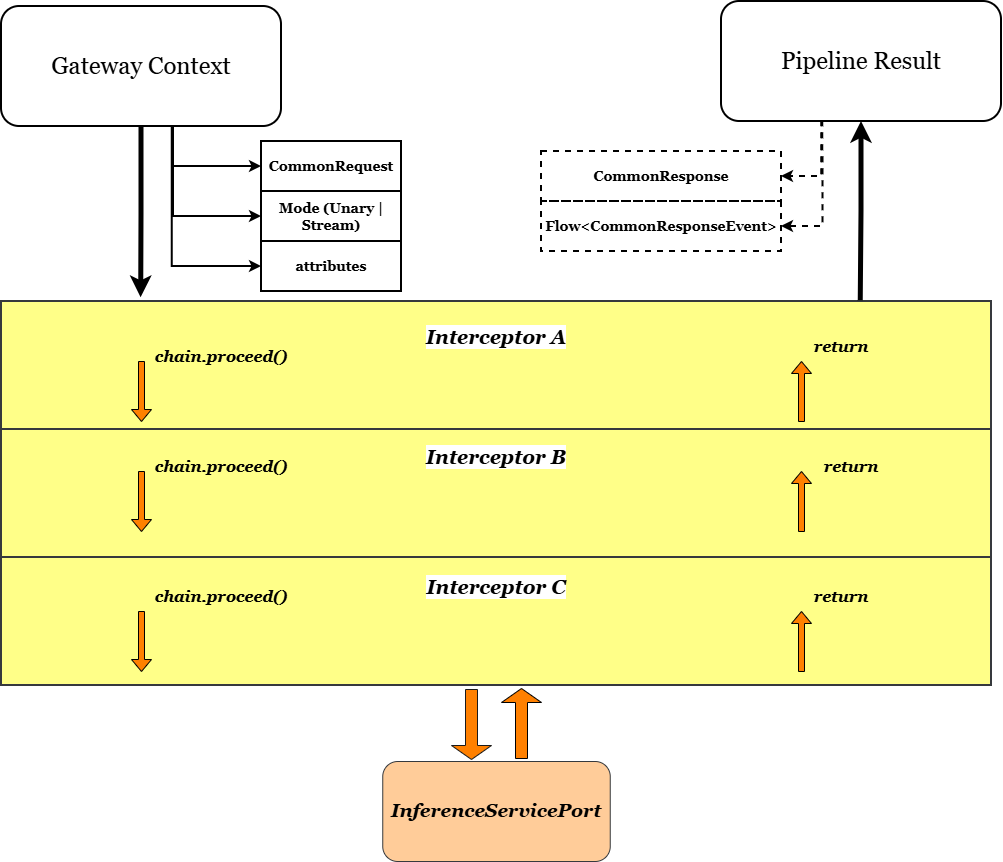
\includegraphics[width=0.9\textwidth]{pipeline.drawio}
        \caption{Visão conceptual da pipeline de interceptors}
        \label{fig:pipeline}
    \end{figure}

    A \textit{pipeline} é composta por \texttt{GatewayPipeline}, \texttt{GatewayPipelineChain}, \texttt{Interceptor} e \texttt{GatewayContext}. O \texttt{GatewayContext} transporta o pedido comum, atributos e modo de execução, podendo representar chamadas síncronas ou \textit{streaming}. A cadeia executa os \textit{interceptors} por ordem e, no fim, invoca o \texttt{DispatcherPort}.

    Esta abordagem melhora a extensibilidade. Um novo comportamento transversal pode ser adicionado como interceptor, sem alterar os adapters ou o dispatcher. Também permite configurar interceptors globais ou específicos por fornecedor, de acordo com as necessidades da aplicação final.

    \section{Arquitetura Interna dos Interceptors}
    O módulo \texttt{interceptors} inclui implementações pré-construídas para preocupações operacionais e de segurança. Todos seguem a mesma ideia base: recebem um \texttt{GatewayContext}, consultam ou acrescentam atributos à \texttt{TypedMap}, decidem se devem chamar \texttt{chain.proceed(context)} e, depois da execução seguinte, podem observar ou transformar o \texttt{PipelineResult}. Esta estrutura permite colocar lógica transversal antes e depois da inferência sem acoplar essa lógica aos adapters de entrada, aos adapters de saída ou ao dispatcher.

    A ordem de execução é configurável. No target JVM, o SDK suporta a anotação \texttt{InterceptorPriority}, usada para executar primeiro interceptors com prioridade superior. No target JavaScript, onde a reflexão sobre anotações é limitada, a ordem segue a sequência definida pela DSL. Assim, comportamentos como autenticação e autorização podem ocorrer no início da cadeia, enquanto métricas, tracing ou logging podem envolver a execução completa.

    \subsection{Interceptor de Telemetria e Observabilidade}
    O \texttt{MetricsInterceptor} é o componente central para a recolha de dados operacionais, sendo crítico para a gestão de performance e visibilidade em sistemas baseados em LLMs. Este interceptor mede o ciclo de vida completo de cada pedido, capturando métricas de latência, sucesso/erro e metadados de execução.

    A implementação distingue-se pelo suporte nativo a \textit{streaming}. Em respostas progressivas, o interceptor não bloqueia a execução; em vez disso, utiliza operadores de fluxo (\texttt{onEach} e \texttt{onCompletion}) para capturar metadados do fornecedor e do modelo à medida que os eventos atravessam a \textit{pipeline}. As métricas são emitidas apenas quando o fluxo é encerrado, garantindo uma medição precisa da duração total da interação (\textit{End-to-End Latency}), mesmo em cenários de resposta longa.

    A arquitetura segue o princípio de inversão de dependência através da porta \texttt{MetricsPort}. O SDK fornece as definições de instrumentos comuns (\texttt{counter}, \texttt{histogram} e \texttt{upDownCounter}), enquanto o adaptador concreto no target JVM mapeia estas chamadas para o ecossistema \textbf{OpenTelemetry}. Esta separação permite que o SDK permaneça agnóstico a ferramentas específicas de monitorização, facilitando a exportação para \textbf{Prometheus}, \textbf{Grafana} ou outros coletores OTLP através da OmniAI Gateway.

    \begin{figure}[H]
        \centering
        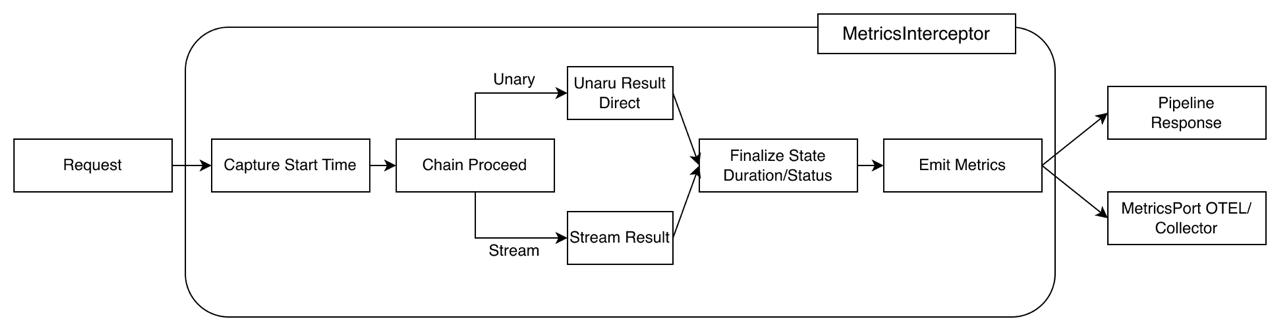
\includegraphics[width=0.9\textwidth]{MetricsInterceptorArch.jpeg}
        \caption{Fluxo interno de processamento e lógica de observabilidade para pedidos unários e streaming}
        \label{fig:p3}
    \end{figure}

    Para adicionar uma métrica, a aplicação usa a DSL do \texttt{gateway-client}. O programador pode ativar a latência padrão, acrescentar atributos globais e definir métricas próprias com uma função \texttt{value}, que extrai o valor a partir do contexto e do resultado, e uma função \texttt{tags}, que acrescenta dimensões de análise.

    \begin{verbatim}
metrics {
    metricsPort = telemetryRuntime.metricsPort
    tracer = telemetryRuntime.tracer

    attributes {
        include(ClientIpMetadataKey, alias = "client.ip")
        attribute("sdk.version") { _, _ -> "1.0.0" }
    }

    defaultLatency {
        enabled = true
        name = "gateway.inference.request.duration"
    }

    customMetrics {
        counter(
            name = "gateway.llm.tokens",
            description = "Total de tokens consumidos",
            unit = "{tokens}"
        ) {
            value { _, result ->
                (result as? PipelineResult.Unary)?.response?.usage?.totalTokens
            }
        }
    }
}
    \end{verbatim}

    Este desenho permite separar três preocupações: a lógica de negócio da métrica, definida na DSL; a recolha no interceptor; e a exportação no adapter de telemetria. Também facilita testes, porque \texttt{NoOpMetricsPort} pode ser usado quando a observabilidade está desligada.

    \begin{figure}[H]
        \centering
        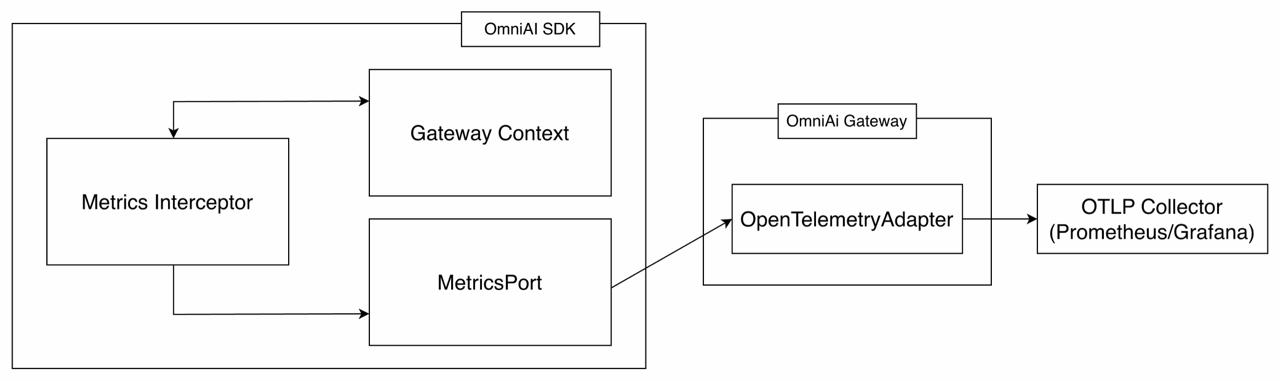
\includegraphics[width=0.9\textwidth]{MetricsGateway.jpeg}
        \caption{observabilidade e métricas operacionais da OmniAI Gateway}
        \label{fig:p3}
    \end{figure}

    \subsection{Interceptor de Autenticação}
    A autenticação é realizada pelo \texttt{AuthenticationInterceptor}, que atua como o primeiro guardião da \textit{pipeline} de segurança. A sua responsabilidade é provar a identidade técnica do chamador antes de permitir que o pedido avance para o \textit{dispatcher}.

    O fluxo inicia-se com a extração do \textit{token} no adapter HTTP a partir do cabeçalho \texttt{Authorization: Bearer <token>}, sendo este propagado para o domínio através de metadados. O interceptor utiliza uma heurística baseada no número de segmentos (separados por pontos) para classificar o \textit{token}: se possuir três segmentos, é tratado como um \textit{JSON Web Token} (JWT); caso contrário, é classificado como um \textit{token} opaco. Esta distinção permite ao sistema selecionar a estratégia de validação adequada, delegando a execução para um \texttt{TokenAuthenticator}.

    No modo \textit{OIDC Discovery} (alinhado com o \textbf{RFC 8414} \cite{rfc8414}), a Gateway obtém dinamicamente os metadados do \textit{Authorization Server} (como o Logto ou Keycloak), incluindo o \textit{issuer}, o \texttt{jwks\_uri} e o \textit{endpoint} de introspeção.

    \begin{figure}[H]
        \centering
        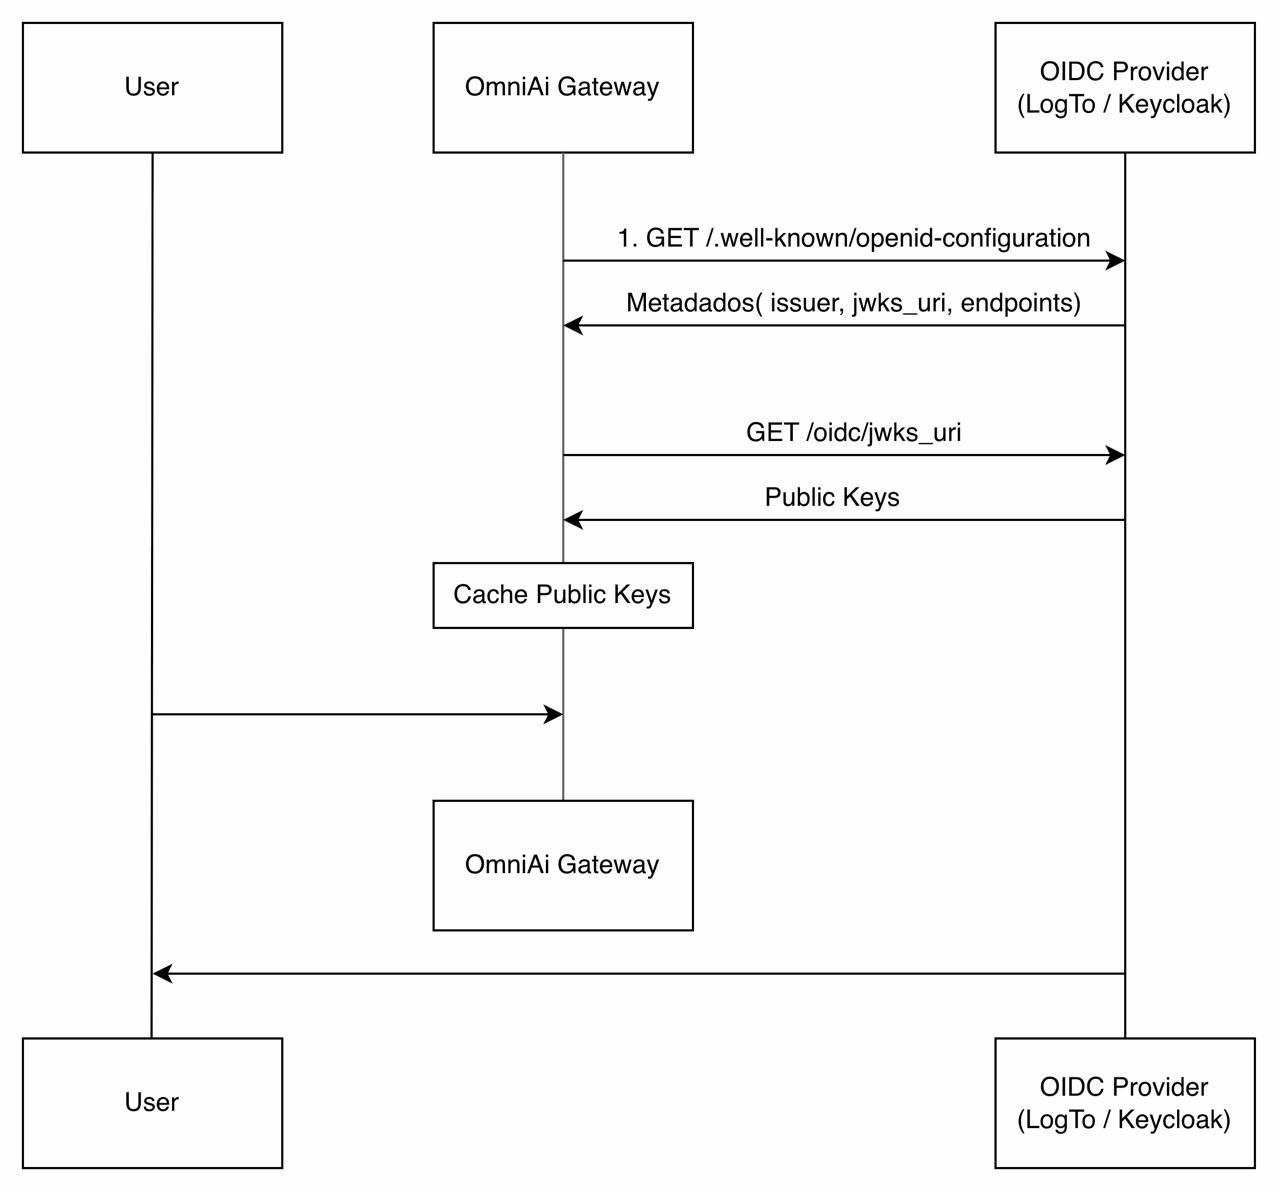
\includegraphics[width=0.9\textwidth]{AutenticationFlow.jpeg}
        \caption{Sequência OIDC: descoberta, JWKS e cache de chaves}
        \label{fig:oidc-sequence}
    \end{figure}

    Para a validação de JWTs (\textbf{RFC 7519} \cite{rfc7519}), o sistema implementa as seguintes etapas:
    \begin{enumerate}
        \item Extração do identificador de chave (\texttt{kid}) do cabeçalho do \textit{token} (\textbf{RFC 7515} \cite{rfc7515}).
        \item Recuperação da chave pública correspondente a partir de um \textit{JSON Web Key Set} (JWKS, \textbf{RFC 7517} \cite{rfc7517}).
        \item Validação da assinatura criptográfica e verificação de \textit{claims} temporais (\texttt{exp}, \texttt{nbf}) e de identidade (\texttt{iss}, \texttt{aud}).
    \end{enumerate}

    Para otimizar este processo e evitar latência excessiva, o \texttt{JwksClient} utiliza uma \textit{cache} de chaves públicas em memória (\texttt{InMemoryKeyCache}). Este componente implementa um mecanismo de rotação de chaves em \textit{background} e um período de \textit{cooldown} (\texttt{minimumTimeToFetchKeys}) que impede o sistema de realizar pedidos repetitivos ao servidor de autorização em caso de chaves não encontradas, mitigando potenciais vetores de negação de serviço (DoS).

    Para \textit{tokens} opacos, a Gateway utiliza o protocolo de \textit{Token Introspection} (\textbf{RFC 7662} \cite{rfc7662}). Dado que este processo exige uma chamada de rede ao \textit{Authorization Server} para cada pedido, a implementação inclui um \texttt{IntrospectionCache} robusto com duas estratégias complementares:
    \begin{itemize}
        \item \textbf{Positive Caching}: Resultados de sucesso (token ativo) são guardados por um período configurável, limitado superiormente pelo tempo de vida (\textit{expiration}) do próprio \textit{token}.
        \item \textbf{Negative Caching}: Resultados de falha (token inválido ou inativo) são guardados por um curto período (\textit{negative TTL}) para prevenir ataques de força bruta.
    \end{itemize}
    Por questões de segurança, os \textit{tokens} opacos são transformados através de um \textit{hash} seguro antes de serem armazenados na \textit{cache}, garantindo que credenciais em texto limpo nunca fiquem expostas na memória do sistema.

    O resultado da validação é encapsulado num \texttt{AuthValidationResult} e armazenado nos atributos do contexto sob a chave \texttt{AUTH\_RESULT\_KEY}. Isto permite que os interceptores seguintes (autorização, métricas, etc.) reutilizem a identidade já apurada sem necessidade de novas validações.

    \begin{figure}[H]
        \centering
        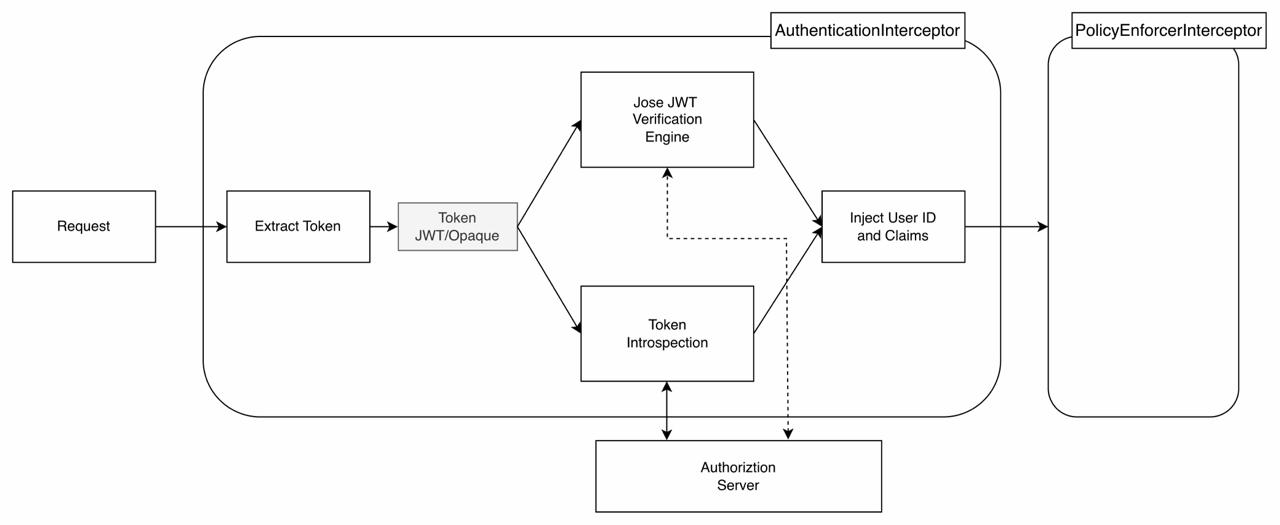
\includegraphics[width=\textwidth]{autenticacao.jpeg}
        \caption{Fluxo interno do interceptor de autenticação}
        \label{fig:auth-interceptor}
    \end{figure}

    A Gateway final usa Logto como Authorization Server local \cite{logto_docs}, executado em Docker juntamente com PostgreSQL, OpenTelemetry Collector, Prometheus e Grafana. A escolha do Logto deveu-se à simplicidade de configuração local, suporte a aplicações Machine-to-Machine e funcionalidades úteis para gerir recursos de API. Também foram realizados testes exploratórios com Keycloak \cite{keycloak_docs}, mas o Logto foi mantido como opção principal por reduzir a complexidade operacional durante o desenvolvimento.

    O script \texttt{run\_claude.py} valida este fluxo num cenário real: abre o browser para autenticação no Logto, usa PKCE para trocar o código por um token e inicia o Claude Code apontando \texttt{ANTHROPIC\_BASE\_URL} para a OmniAI Gateway. Desta forma, um cliente compatível com Anthropic consegue enviar pedidos autenticados através da Gateway.

    \subsection{Interceptor de Autorização}
    A autorização é tratada como uma camada distinta e subsequente à autenticação. Enquanto a autenticação estabelece a identidade do chamador, a autorização determina se essa identidade possui permissão para executar uma operação específica sobre um recurso. No OmniAI SDK, esta lógica é centralizada no \texttt{PolicyEnforcerInterceptor}.

    Este componente segue o modelo arquitetural de referência para autorização centralizada, atuando como um \textit{Policy Enforcement Point} (PEP). A sua função é intercetar o pedido, recolher os atributos necessários e delegar a decisão a um \textit{Policy Decision Point} (PDP) através da porta \texttt{PolicyDecisionPointPort}.

    \begin{figure}[H]
        \centering
        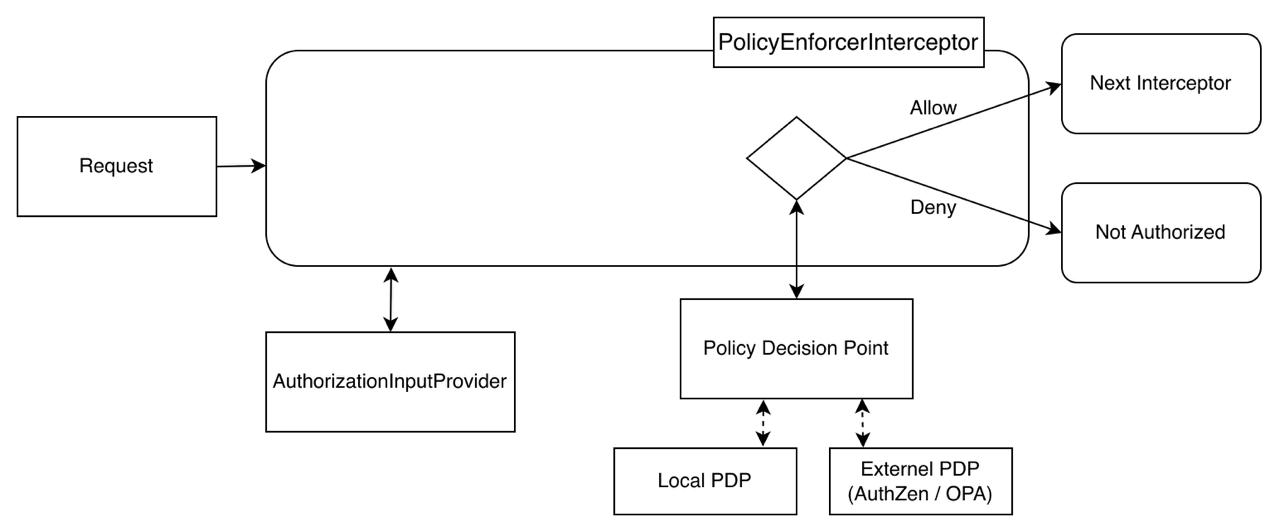
\includegraphics[width=0.9\textwidth]{Authorization.jpeg}
        \caption{Arquitetura do interceptor de autorização: separação entre PEP e PDP}
        \label{fig:authorization-architecture}
    \end{figure}

    O processo de autorização baseia-se num modelo de dados estruturado, designado por \texttt{AuthorizationInput}, que segue o padrão \textbf{Subject-Action-Resource (SAR)}:
    \begin{itemize}
        \item \textbf{Subject}: Representa o utilizador ou aplicação, incluindo o seu identificador, funções (\textit{roles}) e atributos extraídos do \textit{token} validado (via \textit{claims} de JWT ou introspeção).
        \item \textbf{Action}: Define a operação pretendida (ex: \texttt{chat\_completion}, \texttt{list\_models}).
        \item \textbf{Resource}: Identifica o alvo da operação, como o fornecedor (\texttt{openai}, \texttt{anthropic}) ou um modelo específico.
        \item \textbf{Context}: Contém atributos ambientais ou metadados adicionais do pedido, como o endereço IP ou o \textit{timestamp}, que complementam o modelo SAR para decisões contextuais ricas.
    \end{itemize}

    A construção deste \textit{input} é responsabilidade do \texttt{AuthorizationInputProvider}. Esta abstração permite que a Gateway seja extremamente flexível, podendo extrair dados de diversas fontes, como o endereço IP do cliente, o plano de subscrição ou metadados específicos do pedido. Esta riqueza de dados permite implementar políticas de controlo de acesso baseado em atributos.

    A porta do PDP permite integrar diferentes motores de política. O SDK já prevê suporte para o padrão emergente \textbf{AuthZen}, facilitando a integração com servidores de autorização externos e motores de políticas como o \textit{Open Policy Agent} (OPA). Esta separação segue o modelo PEP/PDP/PAP/PIP amplamente utilizado em sistemas de autorização escaláveis \cite{authorization_pips}. Caso o PDP devolva uma decisão de \textit{Deny}, o interceptor interrompe imediatamente a \textit{pipeline}, garantindo que pedidos não autorizados nunca cheguem aos fornecedores de inferência.

    \subsection{Interceptor de Rate Limiting}
    O \texttt{RateLimitInterceptor} aplica limites de utilização antes da chamada ao fornecedor. A lógica é orientada por políticas: cada \texttt{RateLimitPolicy} extrai dados do \texttt{GatewayContext} e devolve um conjunto de \texttt{RateLimitTarget}. Cada target contém uma chave, por exemplo cliente/modelo/plano, e uma \texttt{RateLimitDefinition}, composta por limite, tipo e janela temporal.

    O store atual em memória usa buckets protegidos por \texttt{Mutex}. Quando um pedido chega, o interceptor consome uma unidade de cada bucket aplicável. Se todos permitirem consumo, a pipeline continua. Se algum limite estiver esgotado, o interceptor devolve \texttt{TooManyRequestsError} com \texttt{retryAfter}. Este modelo é adequado para testes e instâncias únicas; numa implantação distribuída, o mesmo contrato \texttt{RateLimitStore} permite substituir a implementação por Redis ou outro backend partilhado.

    \subsection{Interceptor de Circuit Breaker}
    O \texttt{CircuitBreakerInterceptor} protege a Gateway contra chamadas repetidas a um outbound em falha. Para cada combinação de fornecedor/modelo, identifica o \texttt{outbound.key} e consulta o estado no \texttt{CircuitBreakerStore}. Se o circuito estiver \texttt{OPEN}, o pedido falha rapidamente com \texttt{ApiDownError} e o outbound é acrescentado ao conjunto de outbounds negados no contexto.

    Quando a chamada prossegue, o interceptor observa o resultado. Erros incrementam o contador de falhas; ao atingir \texttt{failureThreshold}, o circuito passa para \texttt{OPEN}. Sucessos reiniciam o contador e, quando aplicável, fecham circuitos em \texttt{HALF\_OPEN}. A configuração inclui \texttt{failureThreshold}, \texttt{resetTimeoutMs} e \texttt{halfOpenTestRequests}; a implementação atual cobre a abertura/fecho básico do circuito e deixa a evolução temporal de \texttt{HALF\_OPEN} como ponto natural de melhoria.

    \subsection{Interceptor de Fallback}
    O \texttt{FallbackInterceptor} usa a lista de outbounds disponíveis para tentar alternativas quando a chamada principal falha. Primeiro tenta o outbound correspondente ao fornecedor e modelo pedidos; se falhar, acrescenta esse outbound ao conjunto de negados e tenta os restantes. Para cada tentativa, cria um novo \texttt{GatewayContext} com o mesmo conjunto de atributos, mas com \texttt{provider} e \texttt{model} atualizados para o outbound alternativo.

    A integração com o circuit breaker é feita através do conjunto partilhado de outbounds negados. Assim, se um circuito estiver aberto, o fallback evita esse destino e tenta outro modelo ou fornecedor. Este desenho permite construir políticas de resiliência como ``tentar Gemini, depois OpenAI-compatible via Groq, depois Anthropic'', mantendo a lógica de tentativa fora dos adapters.

    \subsection{Interceptor de Logging e Tracing}
    O \texttt{RequestLoggingInterceptor} regista fornecedor, modelo, sucesso, erro e conclusão de streams através da abstração \texttt{GatewayLogger}. No target JVM, pode ser ligado a SLF4J; no target JS, pode usar consola. O \texttt{TracingInterceptor}, por sua vez, envolve o pedido num span chamado \texttt{gateway.request.process}. Quando combinado com OpenTelemetry, este span permite correlacionar latência, erros, chamadas externas e métricas agregadas.

    \section{MCP Broker e Ferramentas Externas}

    O MCP Broker foi introduzido para separar a gestão de ferramentas externas da lógica específica das APIs de inferência. Em vez de cada adapter conhecer diretamente as ferramentas disponíveis e a forma como estas são executadas, o Broker fornece uma camada intermédia responsável por representar ferramentas, recursos e \textit{prompts} de forma uniforme.

    O módulo inclui abstrações para a definição de ferramentas MCP, modelos de recursos, modelos de \textit{prompts}, geração de esquemas JSON e mapeamento entre o domínio interno e os tipos usados pelo SDK MCP. Esta estrutura permite descrever uma ferramenta através do seu nome, descrição, parâmetros esperados e função de execução, mantendo essa definição separada dos contratos específicos de OpenAI, Anthropic ou Gemini.

    A motivação principal desta abordagem é permitir que o sistema suporte \textit{tool calling} de forma extensível. Embora cada fornecedor represente chamadas de ferramentas de maneira diferente, o domínio comum do OmniAI SDK permite normalizar esses conceitos. Assim, uma ferramenta pode ser descrita uma vez no sistema e posteriormente convertida para o formato esperado por cada fornecedor.

    O desenho do Broker prevê também que, no futuro, as ferramentas possam ser carregadas a partir de ficheiros de configuração, como YAML. Esta capacidade permitiria adicionar, remover ou alterar ferramentas sem recompilar a Gateway, tornando a solução mais flexível para cenários em que diferentes instalações necessitam de conjuntos distintos de ferramentas. No estado atual, o módulo estabelece sobretudo as abstrações e o mapeamento necessários para essa evolução.

    A Figura~\ref{fig:tool-calling} representa o ciclo geral de \textit{tool calling}. Primeiro, o cliente envia um pedido que inclui ou referencia as ferramentas disponíveis. Em seguida, o modelo pode decidir invocar uma dessas ferramentas, devolvendo uma chamada estruturada com o nome da função e os argumentos necessários. A Gateway fica então responsável por executar ou encaminhar essa chamada, recolher o resultado e devolvê-lo ao modelo para que este produza a resposta final.

    Esta separação permite que a execução de ferramentas evolua de forma independente dos adapters de inferência. Dessa forma, novas ferramentas, novos transportes MCP ou novas formas de configuração podem ser integradas sem alterar o núcleo da pipeline nem os contratos principais da Gateway.

    \begin{figure}[H]
        \centering
        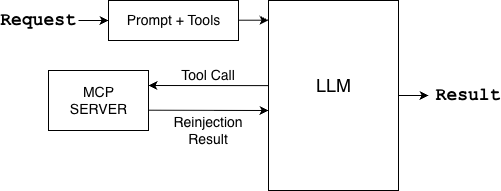
\includegraphics[width=0.45\textwidth]{ToolCallingCycle.png}
        \caption{Representação do ciclo de \textit{tool calling} e interação com ferramentas externas}
        \label{fig:tool-calling}
    \end{figure}

    \section{Distribuição Multiplataforma}

    Um dos objetivos do OmniAI SDK é permitir que a lógica principal da Gateway possa ser reutilizada em diferentes ambientes de execução. Para isso, o projeto foi desenvolvido em Kotlin Multiplatform, com suporte para os targets JVM e JavaScript/Node.js.

    No target JVM, o SDK pode ser utilizado por aplicações Kotlin ou Java. Este é o target mais consolidado no estado atual do projeto, sendo usado pela aplicação \texttt{OmniAiGateway} através de um \textit{composite build} do Gradle. Esta abordagem permitiu validar o SDK numa aplicação real sem exigir uma publicação intermédia. Numa fase posterior, a distribuição poderá ser feita através de um repositório Maven, permitindo que outras aplicações adicionem o SDK como dependência normal.

    No target JavaScript/Node.js, o projeto prepara a exposição de uma API consumível a partir do ecossistema Node.js e TypeScript. Para esse efeito, foi criada uma fachada exportada com \texttt{@JsExport}, permitindo configurar e instanciar componentes da Gateway a partir de código JavaScript. Esta camada tem como objetivo aproximar o SDK de cenários onde a aplicação cliente ou a própria Gateway sejam desenvolvidas em Node.js.

    Apesar desta preparação multiplataforma, a paridade entre JVM e JavaScript ainda não é total. Algumas partes do runtime, como transporte HTTP, integração com mecanismos de segurança, observabilidade e montagem completa da Gateway, ainda exigem consolidação no target JavaScript. Assim, a distribuição via NPM deve ser entendida como uma linha de evolução preparada pela arquitetura, mas ainda não totalmente finalizada.

    Esta decisão arquitetural permite separar o núcleo comum do SDK dos detalhes específicos de cada plataforma. O domínio, os contratos, a pipeline e parte da lógica de configuração podem ser partilhados, enquanto componentes dependentes do ambiente de execução podem ter implementações próprias em JVM ou JavaScript. Desta forma, o projeto mantém uma base comum reutilizável e abre caminho para futuras distribuições em Maven e NPM.

    \chapter{Provas de Conceito (PoCs) e Validação}

    \section{Demonstração de Roteamento Inteligente}
    A validação da Gateway foi feita através de uma aplicação Ktor que consome o OmniAI SDK e expõe endpoints compatíveis com OpenAI, Anthropic e Gemini. A configuração permite ativar fornecedores individualmente e definir um ou mais modelos por fornecedor. A resolução de modelos segue precedência entre variáveis de ambiente, listas em ficheiro de configuração e valores simples.

    O roteamento atual demonstra a seleção de fornecedores configurados e fornece a base para políticas mais avançadas. O trabalho desenvolvido em \textit{fallback} e \textit{circuit breaker} permite evoluir o roteamento para considerar falhas, indisponibilidade e degradação de modelos.

    \section{Invocação de Ferramentas via MCP}
    O estudo das APIs de inferência permitiu mapear as diferenças de \textit{tool calling} entre OpenAI, Anthropic e Gemini. A OpenAI devolve argumentos como strings JSON em \texttt{tool\_calls}; a Anthropic usa blocos \texttt{tool\_use} e \texttt{tool\_result}; a Gemini usa \texttt{functionCall} e \texttt{functionResponse}. O domínio comum do SDK normaliza estes conceitos para \texttt{CommonTool}, \texttt{ToolChoice} e eventos de chamada de ferramenta.

    Esta normalização é essencial para o MCP Broker, porque permite que uma ferramenta seja definida uma vez e exposta a diferentes modelos, mesmo quando cada fornecedor espera um formato próprio de descrição e execução.

    \section{Validação com Aplicações Cliente}
    Foram estudados cenários de integração com aplicações que permitem alterar o endpoint da API, como ferramentas compatíveis com OpenAI, LibreChat, Dify e Claude Code. O objetivo destes cenários é demonstrar que a Gateway pode ser introduzida entre a aplicação cliente e o fornecedor sem alterar a lógica principal do cliente.

    No caso do Claude Code, foi criado um \textit{bootstrap} em Python, \texttt{run\_claude.py}, que abre o fluxo de autenticação no browser contra o Logto, usa PKCE para obter um token e inicia o Claude Code com \texttt{ANTHROPIC\_BASE\_URL} a apontar para a Gateway. O script também injeta o cabeçalho \texttt{Authorization} para testar a passagem do JWT pela Gateway.

    Também foi criado um teste em Node.js com o SDK oficial da Anthropic, configurado com \texttt{baseURL} local e chave fictícia, para validar que clientes existentes conseguem direcionar pedidos para a OmniAI Gateway quando esta expõe um contrato compatível.

    \chapter{Conclusões e Trabalho Futuro}

    \section{Conclusões}
    O projeto evoluiu de uma Gateway específica para um SDK reutilizável capaz de instanciar gateways de IA configuráveis. Esta evolução tornou a solução mais alinhada com o problema identificado: reduzir acoplamento entre aplicações cliente e fornecedores de LLMs, centralizando contratos, autenticação, autorização, observabilidade, resiliência e integração com ferramentas.

    O OmniAI SDK demonstra que é possível definir um domínio comum para pedidos, respostas, eventos de \textit{streaming} e ferramentas, mantendo adapters específicos para OpenAI, Anthropic e Gemini. A Arquitetura Hexagonal ajudou a manter esta separação, enquanto a \textit{pipeline} de \textit{interceptors} permitiu adicionar comportamentos transversais sem contaminar o domínio.

    A OmniAI Gateway, construída sobre o SDK, valida a proposta através de uma aplicação real em Ktor, configurável por ficheiro e variáveis de ambiente, com suporte para telemetria e integração com um Authorization Server. Esta aplicação mostra que o SDK pode ser usado para criar rapidamente uma API Gateway robusta para cenários de IA.

    \section{Melhorias Futuras e Escalabilidade}
    Como trabalho futuro, existem várias linhas de evolução. A primeira é consolidar a distribuição pública do SDK via Maven e NPM, garantindo documentação de instalação, versionamento semântico e exemplos de consumo. A segunda é completar a paridade entre targets JVM e JavaScript, sobretudo na montagem de runtime e transporte HTTP.

    Outra melhoria importante é aprofundar o MCP Broker, incluindo carregamento efetivo de ferramentas via YAML, execução completa dos handlers MCP e suporte robusto a SSE e WebSocket. Também será relevante melhorar as políticas de roteamento, permitindo decisões com base em custo, latência, disponibilidade, qualidade do modelo, plano do cliente e limites de utilização.

    Por fim, a camada de segurança pode evoluir para políticas de autorização mais expressivas, integração com PDPs externos, introspeção real de tokens opacos e mapeamento mais fino entre claims, planos e quotas. Estas melhorias permitiriam aproximar a OmniAI Gateway de uma solução pronta para ambientes multi-tenant e produção.

% ================= APÊNDICES =================
    \appendix

    \chapter{Histórico de Planeamento e Riscos}
    Durante a fase de planeamento foram identificados riscos técnicos e operacionais que continuam relevantes para a evolução do projeto.

    \section{Riscos}

    Durante o desenvolvimento do projeto foram identificados vários riscos técnicos e operacionais. Estes riscos influenciaram decisões de desenho, prioridades de implementação e estratégias de validação.

    \begin{itemize}
        \item \textbf{Curva de aprendizagem tecnológica:}
        O projeto exigiu a utilização de tecnologias e conceitos com elevada complexidade, nomeadamente Kotlin Multiplatform, arquitetura hexagonal, APIs de inferência de diferentes fornecedores, autenticação baseada em OIDC/OAuth2 e o Model Context Protocol. Esta diversidade tecnológica representou um risco inicial, porque aumentou o tempo necessário para compreender os contratos externos, configurar o ambiente de desenvolvimento e definir uma arquitetura estável.
        A mitigação passou pela realização de protótipos incrementais, pelo estudo isolado das APIs de OpenAI, Anthropic e Gemini, e pela separação progressiva do sistema em módulos com responsabilidades claras.

        \item \textbf{Instabilidade de serviços externos:}
        A Gateway depende de serviços de terceiros, como APIs de inferência, servidores de autorização e ferramentas externas. Estes serviços podem apresentar indisponibilidade temporária, alterações nos contratos, limites de utilização ou comportamentos diferentes dos documentados. Este risco poderia comprometer a validação da solução e tornar os testes dependentes de fatores externos.
        Para reduzir este impacto, foram usados testes locais, servidores simulados, mocks e abstrações sobre o transporte HTTP. Além disso, a arquitetura inclui mecanismos de resiliência, como \textit{fallback} e \textit{circuit breaker}, que permitem lidar melhor com falhas de fornecedores.

        \item \textbf{Custos de utilização:}
        A execução de testes com modelos pagos pode gerar custos inesperados, especialmente em cenários de \textit{streaming}, chamadas repetidas ou testes de integração. Este risco é relevante porque a Gateway incentiva a experimentação com múltiplos fornecedores e modelos.
        A mitigação passou por limitar o número de chamadas reais, utilizar fornecedores com quotas gratuitas sempre que possível, recorrer a testes locais e validar grande parte da lógica através de contratos, adapters e servidores simulados.

        \item \textbf{Complexidade de normalização entre fornecedores:}
        As APIs de OpenAI, Anthropic e Gemini partilham conceitos semelhantes, como mensagens, modelos, parâmetros de geração e ferramentas, mas representam esses conceitos de formas diferentes. Alguns elementos, como \textit{tool calling}, \textit{streaming}, multimodalidade e metadados específicos, não têm correspondência direta entre fornecedores.
        Este risco poderia levar a uma abstração demasiado rígida ou à perda de informação específica de cada API. Para o mitigar, foi definido um domínio comum extensível, complementado por campos de opções específicas do fornecedor. Desta forma, o SDK consegue representar o núcleo comum sem impedir a passagem de características particulares de cada API.

        \item \textbf{Segurança e dados sensíveis:}
        A centralização dos pedidos numa Gateway aumenta a responsabilidade sobre autenticação, autorização, gestão de tokens, logs, métricas e chaves de API. Um erro nesta camada poderia expor dados sensíveis ou permitir acesso indevido a modelos e recursos.
        A mitigação passou pela introdução de uma pipeline de segurança com autenticação e autorização separadas, validação de tokens, integração com um Authorization Server e cuidado na recolha de métricas e logs. Ainda assim, este risco continua relevante para uma evolução futura em direção a ambientes de produção e cenários multi-tenant.

        \item \textbf{Âmbito e complexidade funcional:}
        O domínio das Gateways de IA inclui várias funcionalidades possíveis, como roteamento por custo, políticas avançadas de autorização, execução automática de ferramentas, suporte completo a MCP, cache semântica e gestão de quotas por utilizador. Implementar todas estas capacidades numa primeira versão aumentaria significativamente o risco de atrasos e instabilidade.
        A mitigação passou pela definição de um âmbito inicial mais controlado, focado na arquitetura base, nos adapters principais, na pipeline de interceptors e numa Gateway funcional construída sobre o SDK. As funcionalidades mais avançadas foram identificadas como trabalho futuro.
    \end{itemize}

    \section{Planeamento}
    \begin{table}[H]
        \centering
        \footnotesize
        \renewcommand{\arraystretch}{1.2}
        \begin{tabular}{|c|l|p{11.0cm}|}
            \hline
            \textbf{Semana} & \textbf{Período} & \textbf{Descrição} \\
            \hline
            1 & 18 fev -- 22 fev (parcial) & Estudo das APIs de inferência e protocolo MCP. \\
            2 & 23 fev -- 1 mar & Continuação da semana anterior e início da proposta. \\
            3 & 2 mar -- 8 mar & \textbf{Entrega Proposta do projeto} \\
            4 & 9 mar -- 15 mar & Configuração inicial da biblioteca, definição da arquitetura base e das interfaces. \\
            5 & 16 mar -- 22 mar & Integração com as APIs de inferência. Foco inicial em dois fornecedores estáveis. \\
            6 & 23 mar -- 29 mar & Integração do MCP no OmniAI Core. Invocação e registo dinâmico de ferramentas, gerindo o ciclo de \textit{tool calling}. \\
            7 & 30 mar -- 5 abr & Implementação do roteamento inteligente de modelos (otimização de custos) e mecanismos de redundância (\textit{fallback} e \textit{retry}). \\
            8 & 6 abr -- 12 abr & Implementação dos mecanismos de segurança, como controlo de acesso, preparação do contexto e remoção de dados sensíveis. \\
            9 & 13 abr -- 19 abr & Conclusão das implementações anteriores. \\
            10 & 20 abr -- 26 abr & \textbf{Apresentação de Progresso} \\
            11 & 27 abr -- 3 mai & Início do desenvolvimento da aplicação final OmniAI Gateway. Exposição da WEB API. \\
            12 & 4 mai -- 10 mai & Continuação da semana anterior e integração do MCP na OmniAI Gateway. \\
            13 & 11 mai -- 17 mai & Término de todas as APIs de comunicação para o exterior. \\
            14 & 18 mai -- 24 mai & Testes de integração do Core e da Gateway. \\
            15 & 25 mai -- 31 mai & \textbf{Entrega da Versão beta} \\
            16 & 1 jun -- 7 jun & Refinamento de testes a todos os módulos. \\
            17 & 8 jun -- 14 jun & Refinamento de código, desempenho e limpeza de bugs do sistema. \\
            18 & 15 jun -- 21 jun & Continuação da semana anterior e refinamento do relatório final. \\
            19 & 22 jun -- 28 jun 2026 & Conclusão do relatório final. \\
            20 & 29 jun -- 5 jul 2026 & Vistoria completa a todo o sistema e polimento de falhas para a entrega da Versão final. \\
            21 & 6 jul -- 11 jul 2026 (parcial) & \textbf{Entrega Final do Projeto e Relatório} \\
            \hline
        \end{tabular}
        \caption{Planeamento semanal do projeto}
    \end{table}
% ================= BIBLIOGRAFIA =================
    \renewcommand{\bibname}{Referências}
    \bibliographystyle{IEEEtran}
    \bibliography{references}

\end{document}
